\begin{song}{title=\predtitle\centering Dům u vycházejícího Slunce \\\large \vspace*{-0.3cm}}  %% sem se napíše jméno songu a autor
\begin{centerjustified}
\nejvetsi

\sloka
Snad ^{Ami}znáš ten ^{C}dům za ^{Dmi}New ^{F}Orleans,

ve ^{Ami}štítu ^{C}znak Slunce ^{E}má,

je to ^{Ami\z}dům,~kde ^{C}lká sto ^{Dmi}chlapců ^{F}ubohých

a ^{Ami\z}v~němž ^{E}jsem zkejs' i ^{Ami E}já.~~~~~

\sloka
Mý mámě Bůh dal věnem

jen prát a šít blue jeans,

táta můj se flákal jen

sám po New Orleans.

\sloka
Bankrotář se zhroutil před hernou,

jenom bídu svou měl a chlast,

k putykám pak táh' tu pouť mizernou

a znal jenom pít a krást.

\sloka
Být matkou, tak dám svým synům

lepší dům, než má kdo z vás,

ten dům, kde spím, má emblém sluneční,

ale je v něm jen zima a mráz.

\sloka
Kdybych směl se hnout z těch kleští,

pěstí vytrhnout tu mříž,

já jak v snách bych šel do New Orleans

a měl tam k Slunci blíž.



\end{centerjustified}
\setcounter{Slokočet}{0}
\end{song}

%\begin{figure}[h]
%\predtitle\centering
%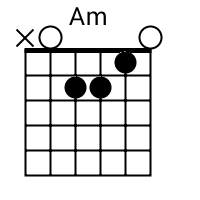
\includegraphics[width=3cm]{../Akordy/am.png}
%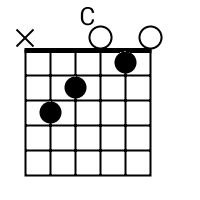
\includegraphics[width=3cm]{../Akordy/c.png}
%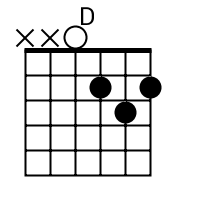
\includegraphics[width=3cm]{../Akordy/d.png}
%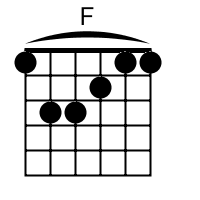
\includegraphics[width=3cm]{../Akordy/f.png}
%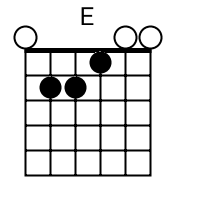
\includegraphics[width=3cm]{../Akordy/e.png}
%\end{figure}
